\subsubsection{Sunquake Literature Review}
The idea that solar flares can cause acoustic waves inside the Sun was originally put forward by \citep{1972ApJ...176..833W}. Wolff made the connection that a large solar flare releasing enough energy to heat the photosphere, would generate expansion of photospheric material, which could lead to an impulsive stimulation of oscillations in the Sun's interior. Wolff also commented that it would be difficult to observe interior oscillations with current (in the 1970s) solar velocity measurement techniques.

A little over twenty years later and Wolff's idea was built upon by \cite{1995ESASP.376b.341K}, who showed theoretically that acoustic waves in the solar interior could be generated by a large solar flare, and that they may be detectable. A year later and the first detection of a sunquake was made by \cite{1998Natur.393..317K} during an X class solar flare on July the 9th 1996. Their observational data came from the Solar and Heliospheric Observatory (SOHO) via the Michelson Doppler Imager (MDI) which images the movement of photospheric material by analysing shifts in wavelength of the emitted light. They observed a prominent impulsive downward signature in the Dopplergrams directly over a compact point source which subsequently emanates a set of concentric acoustic waves (see Figure \ref{mdiquake96}). The timing of maximum downward velocity of material derived from the Dopplergrams was out of sync with peak hard x-ray measurements by around a minute. This time delay, coupled with white-light enhancement in the lower atmosphere led to the conclusion that during the flare, accelerated energetic particles heat the cool dense chromosphere causing a shock front which travels downward, depositing energy in lower atmospheric layers, generating a sunquake.

\begin{figure}[hb]
  \begin{center}
  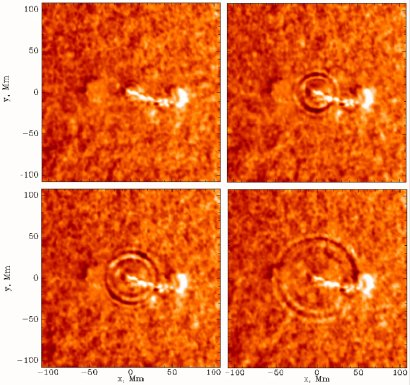
\includegraphics[width=0.80\textwidth]{soho-mdi-quake-96}
\caption{\cite{1998Natur.393..317K} produced SOHO MDI Dopplergrams from the 1996 July 9th, X class solar flare showing the sunquake expanding outward from it's seismic epicentre to a radial distance of $1.2\times10^{8}$ metres. Wave-fronts accelerate from a velocity of 30km/s to 100km/s}\label{mdiquake96}
\end{center}
\end{figure}


The first sunquake observation opened up a whole new area of solar physics, leading to subsequent detections associated other flares. The majority of observations show that sunquakes are often the product of highly impulsive flares, with the acoustic source aligning spatially with white light enhancement in the lower solar atmosphere and hard x-ray emission in the upper-atmosphere \citep{2005ApJ...630.1168D, 2007ApJ...664..573Z}. \cite{2005ApJ...630.1168D} went on to calculate the energy needed to stimulate the propagation of an acoustic wave in the sub-photosphere, finding that only $\sim10^{-3}$ of the energy released by a flare is enough to generate a sunquake. This was an important calculation because it forced the solar community to consider that it might be possible for low energy flares to produce sunquakes, leading to subsequent work by \cite{2008SoPh..251..613M} looking at seismicity of M-class flares.

A paper by \cite{2000ApJ...531L..75H} put forward for the first time, that sunquake production may depend on the changing configuration of the local magnetic field. This idea was further reinforced by \cite{2001ApJ...550L.105K} reporting observations of impulsive changes in magnetic field strength at the photosphere during a solar flare. These magnetic transients were shown to approximately correlate in time and space with hard x-rays, impulsive increases in plasma velocity and increased emission. This line of study was continued \citep{2009MNRAS.395L..39M}, investigating the magnetic field variation of the photosphere in many flares. The study found that some flares with seismicity do not have a spatial and temporal correlation between sunquakes and magnetic transients. Some flares have magnetic transients and no seismicity, and some flares have a good co-spatial alignment of acoustic activity and magnetic variability. It was noted that the impulsiveness of the magnetic field variation could be important as to whether a sunquake is generated.

Some of the most intriguing of sunquake observations are those that do not abide by the usual set of observable features, in that they are not necessarily associated with hard x-rays and excess white-light emission. For example, a statistical survey carried out by \cite{2012SoPh..277..317P}, highlighted a flare containing three footpoints with a seismic source that was co-temporal but not co-spatial with it's closest HXR footpoint; and another source which was co-spatial and co-temporal with its nearest HXR footpoint. This showed that a sunquake does not necessarily correlate with locations of peak emission. Another example by \cite{2011ApJ...741L..35Z} reports an observation of two seismic sources associated with footpoints of an erupting flux rope. During the eruption, the magnetic field above each seismic source undergoes an abrupt permanent reconfiguration. The authors cite the possibility that there exists particle beams low enough in population that HXR emission is undetectable. Further papers investigating the same event \citep{2013SoPh..284..315Z} show that there are downward motions of material above the seismic sources and that energy provided by magnetic transients may not be able to account for the acoustic power generated. These observational oddities prove that mechanisms that generate sunquakes are not well understood and there is much research to be done to classify the different progenitors.

